\documentclass[12pt,a4paper]{report}
\usepackage[utf8]{inputenc}
\usepackage[english,russian]{babel}
\usepackage{indentfirst}
\usepackage{pdfpages}
\usepackage{titlesec}
\usepackage{listings}
\usepackage{amsmath}

% Вставка картинки
\usepackage{graphicx}
\graphicspath{{schemes/}}
\DeclareGraphicsExtensions{.pdf,.png,.jpg}

\usepackage[14pt]{extsizes}

\newcommand{\hsp}{\hspace{20pt}}
\titleformat{\chapter}[hang]{\large\bfseries}{\thechapter{. }}{0pt}{\large\bfseries}
\titlelabel{hlabel-formati}
\titlespacing{\chapter}{42pt}{-20pt}{12pt}
\titleformat{\section}[hang]{\large\bfseries}{\thesection{. }}{0pt}{\large\bfseries}
\titlespacing{\section}{42pt}{12pt}{5pt plus 5pt}

% Отступ абзаца
\usepackage{indentfirst}
\setlength{\parindent}{1.5cm}

% Межстрочный интервал
\usepackage{setspace}
\onehalfspacing % интервал 1.5

\usepackage[left=3cm, right=1cm, top=2cm, bottom=2cm]{geometry}

\begin{document}
% Титульник
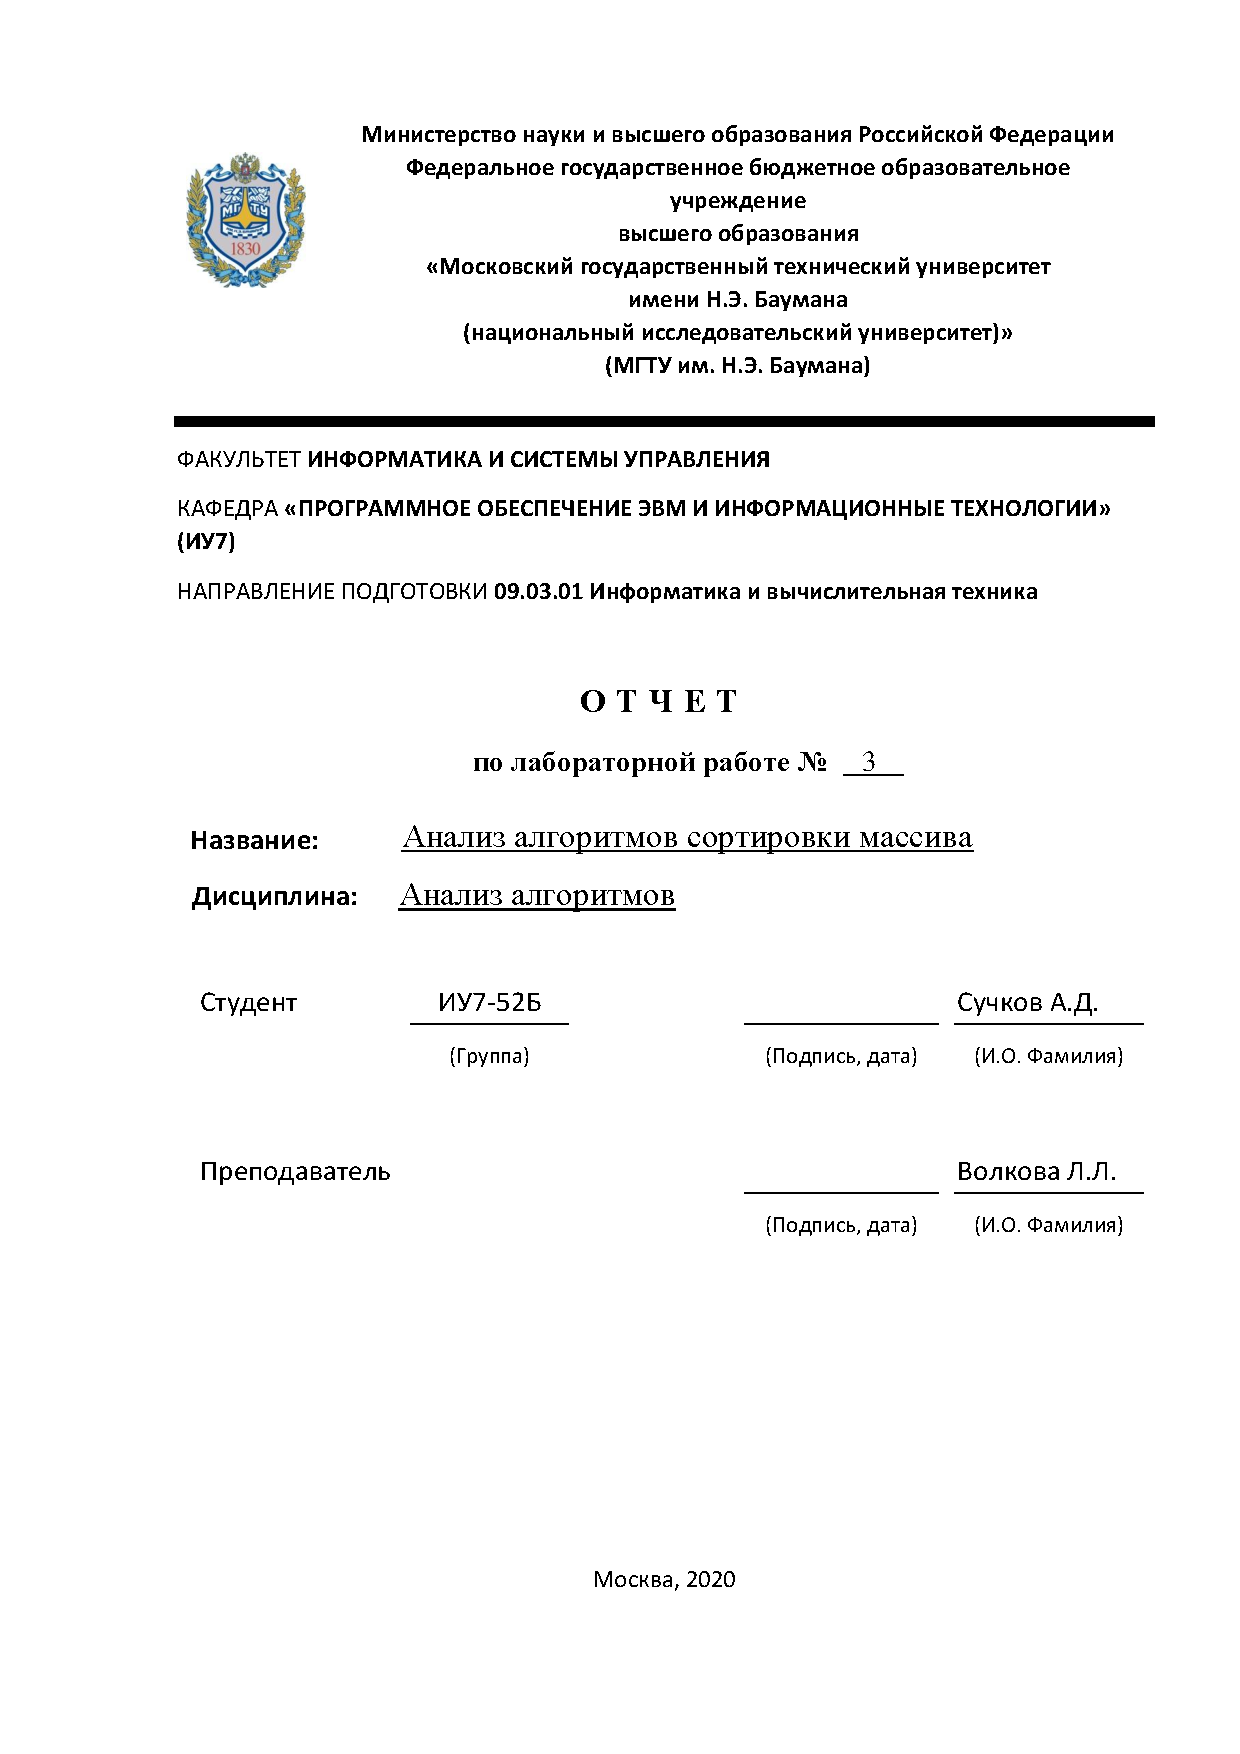
\includepdf[pages=1]{titul.pdf}
% Оглавление
\tableofcontents

\newpage
\chapter*{Введение}
\addcontentsline{toc}{chapter}{Введение}

\textbf{Сортировка массива} -- одна из самых популярных и востребованных операций над массивами.
Массив -- структура данных, которая хранит набор значений (элементов массива), идентифицируемых по индексу или набору 
индексов, принимающих целые (или приводимые к целом) значения из некоторого заданного непрерывного диапазона.

Алгоритмы сортировок реализуют упорядочивание элементов в списке. В случае, когда элемент списка имеет несколько 
полей, поле, служащее критерием порядка, будет называться ключом сортировки. 
На практике в качестве ключа часто выступает число, в то время как остальные поля не участвуют в работе алгоритма.

С каждым годом объёмы хранилищ данных стремительно увеличиваются и поэтому от алгоритмов сортировок требуется 
максимальная производительность.

\newpage
\chapter{Аналитическая часть}

Цель данной лабораторной работы заключается в изучении алгоритмов сортировки массивов. 
Рассматриваются алгоритмы сортировки пузырьком, вставками и шейкерная сортировка. 
Требуется рассчитать и изучить трудоёмкость и затрачиваемое каждым алгоритмом время. \\

Можно выделить следующие задачи лабораторной работы:
\begin{itemize}
    \item изучить работу алгоритмов сортировки;
    \item выполнить полную математическую оценку трудоёмкости для алгоритмов сортировки с указанием лучшего и худшего случаев;
    \item реализовать три алгоритма сортировки;
    \item сравнить работу алгоритмов сортировок и сделать выводы.  
\end{itemize}

\section{Сортировка пузырьком}

Алгоритм состоит из повторяющихся проходов по сортируемому массиву. 
За каждый проход элементы последовательно сравниваются попарно и, если порядок в паре неверный, выполняется обмен элементов. 
Проходы по массиву повторяются N-1 раз или до тех пор, пока на очередном проходе не окажется, что обмены больше не нужны, что 
означает -- массив отсортирован. \\

При каждом проходе алгоритма по внутреннему циклу, очередной наибольший элемент массива ставится на своё место в конце массива 
рядом с предыдущим «наибольшим элементом», а наименьший элемент перемещается на одну позицию к началу массива («всплывает» до 
нужной позиции, как пузырёк в воде — отсюда и название алгоритма). \\

\section{Сортировка вставками}

Алгоритм сортировки, в котором элементы входной последовательности просматриваются по одному, и каждый новый поступивший 
элемент размещается в подходящее место среди ранее упорядоченных элементов. \cite{analyse2_info} \\

В начальный момент отсортированная последовательность пуста. 
На каждом шаге алгоритма выбирается один из элементов входных данных и помещается на нужную позицию в уже отсортированной 
последовательности до тех пор, пока набор входных данных не будет исчерпан. 
В любой момент времени в отсортированной последовательности элементы удовлетворяют требованиям к выходным данным алгоритма. \\

\section{Шейкерная сортировка}

Шейкерная сортировка -- разновидность пузырьковой сортировки. \cite{analyse1_info}
Анализируя метод пузырьковой сортировки, можно отметить два обстоятельства.
Во-первых, если при движении по части массива перестановки не происходят, то эта часть массива уже отсортирована и, следовательно, 
её можно исключить из рассмотрения.
Во-вторых, при движении от конца массива к началу минимальный элемент «всплывает» на первую позицию, а максимальный элемент 
сдвигается только на одну позицию вправо.
Эти две идеи приводят к следующим модификациям в методе пузырьковой сортировки. \\

Границы рабочей части массива (то есть части массива, где происходит движение) устанавливаются в месте последнего обмена на каждой 
итерации. 
Массив просматривается поочередно справа налево и слева направо.

\section{Вывод}

Таким образом, были рассмотрены алгоритмы сортировки пузырьком, вставками и шейкерная сортировка.
Также разобраны принципы работы этих алгоритмов.

\newpage
\chapter{Конструкторская часть}

\section{Требования к программе}

Для дальнейшего тестирования программы необходимо обеспечить консольный ввод размера массива и его элементов, а также обеспечить 
выбор алгоритма сортировки.
На выходе должны получить отсортированный массив.
Также необходимо реализовать функцию подсчёта процессорного времени, которое могут затрачивать функции.

\section{Схемы алгоритмов}

На рисунках 2.1 - 2.5 приведены схемы алгоритмов сортировки массива.

\begin{figure}[h]
    \center{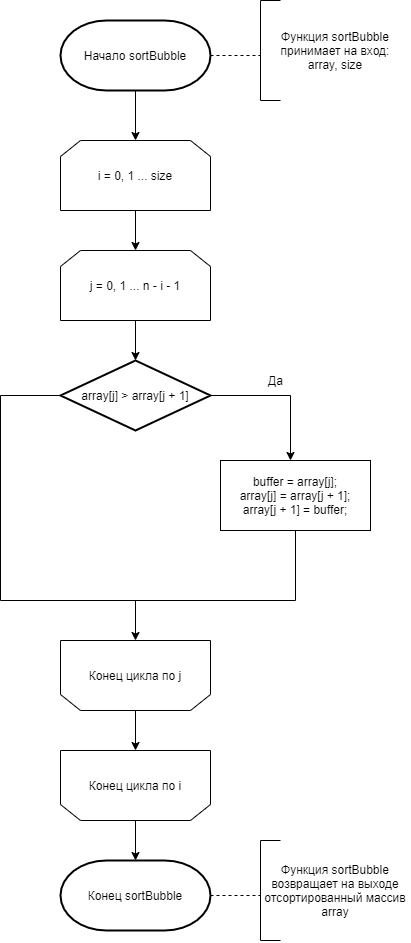
\includegraphics[scale=0.6]{scheme_bubble}}
    \caption{Схема сортировки пузырьком}
    \label{fig:image}
\end{figure}

\begin{figure}[h]
    \center{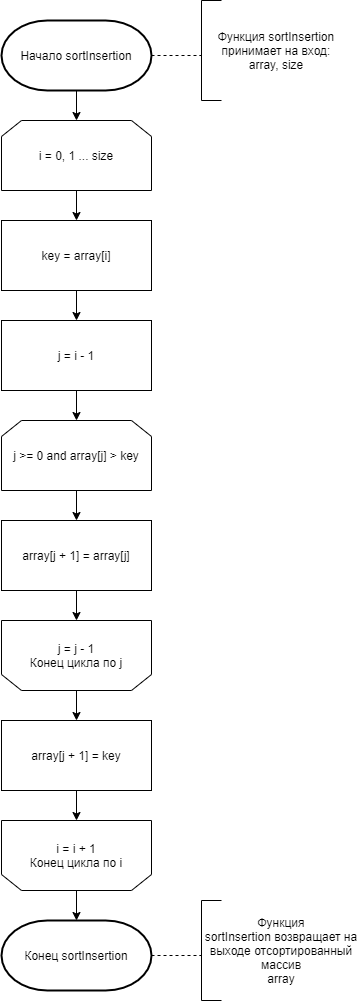
\includegraphics[scale=0.6]{scheme_insert}}
    \caption{Схема сортировки вставками}
    \label{fig:image}
\end{figure}

\begin{figure}[h]
    \center{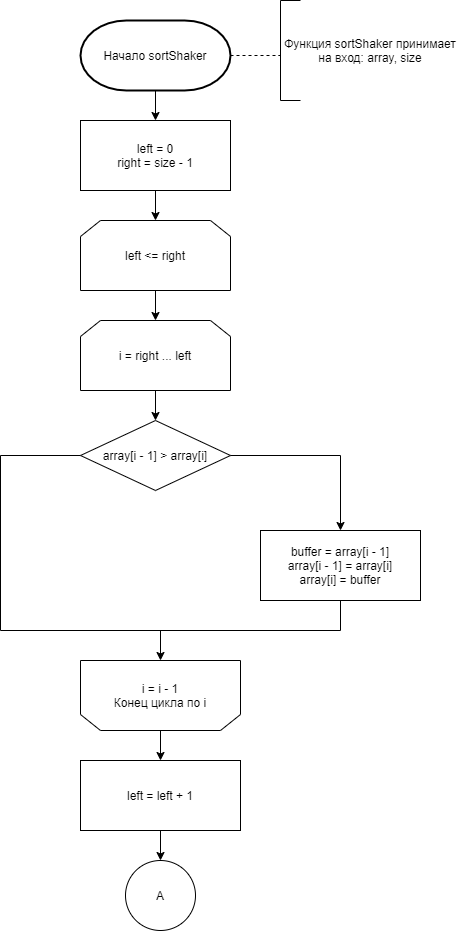
\includegraphics[scale=0.6]{scheme_shaker_p1}}
    \caption{Схема шейкерной сортировки, часть 1}
    \label{fig:image}
\end{figure}

\begin{figure}[h]
    \center{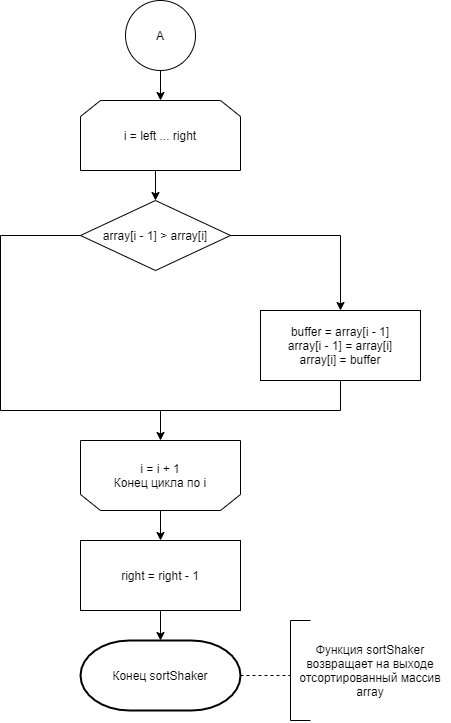
\includegraphics[scale=0.6]{scheme_shaker_p2}}
    \caption{Схема шейкерной сортировки, часть 2}
    \label{fig:image}
\end{figure}

\section{Подсчёт трудоёмкости алгоритмов}

Введём модель вычисления трудоёмкости для оценки алгоритмов:
%\begin{itemize}
%    \item базовые операции стоимостью 1 -- $+, -, *, /, =, ==, <=, >=, !=, +=, []$;
%    \item оценка трудоёмкости цикла: $F_{cycle} = init + N \cdot (a + F_{body} + post) + a$, где a - условие цикла, init - предусловие цикла, post - постусловие цикла;
%    \item стоимость условного перехода применим за 0, стоимость вычисления условия остаётся
% \end{itemize}

\begin{itemize}
    \item базовые операции стоимостью 1 -- $+, -, \cdot , /, =, ==, <=, >=, !=, +=, []$;
    \item оценка трудоёмкости цикла for от 0 до N с шагом 1 $F_{for} = 2 + N \cdot (2 + F_{body})$, где $F_{body}$ -- тело цикла;
    \item стоимость условного перехода примем за 0, стоимость вычисления условия остаётся. 
\end{itemize}

%Далее можно подсчитать и оценить трудоёмкость каждого из алгоритмов сортировки. \\

Оценим трудоёмкость алгоритмов сортировки массива по коду программы.

\textbf{Сортировка пузырьком} \\

%Лучший случай - $2 + (N - 1) \cdot (3 + 1 + 2 + (N / 2) \cdot 8) = 4NN + 2N - 6$

%Худший случай - $2 + (N - 1) \cdot (3 + 1 + 2 + (N / 2) \cdot (8 + 9)) = 8,5NN - 2,5N - 4$ \\

Лучший случай -- $2 + 2 \cdot N + 3 \cdot N \cdot N$

Худший случай -- $2 + 2 \cdot N + 6 \cdot N \cdot N$ \\

\newpage
\textbf{Сортировка вставками} \\

%Лучший случай - $2 + N \cdot (2 + 2 + 3 + 6) = 13N + 2$

%Худший случай - $2 + N \cdot (2 + 2 + 3 + 6 + (N - 1) / 4 \cdot (5 + 4)) = 4,5NN + 8,5N + 2$ \\

Лучший случай -- $2 + 9 \cdot N + 7/2 \cdot N \cdot N$

Худший случай -- $2 + 2 \cdot N + 11/2 \cdot N \cdot N$ \\

\textbf{Шейкерная сортировка} \\

Лучший случай -- $12 \cdot N \cdot N + 7 \cdot N + 5$

Худший случай -- $28 \cdot N \cdot N + 7 \cdot N + 5$

\section{Вывод}

Таким образом, выше были сформированы требования к программе и составлены схемы алгоритмов.
Также подсчитана трудоёмкость для каждого их алгоритмов.

\newpage
\chapter{Технологическая часть}

\section{Выбор языка программирования}

В качестве языка программирования было решено выбрать C++, так как уже имеется опыт работы с библиотеками и 
инструментами языка, которые позволяют реализовать и провести исследования над алгоритмами сортировки массивов.

\section{Реализация алгоритмов}

В листингах 3.1 - 3.3 приведены реализации алгоритмов сортировки массивов на ЯП C++. \\

\textrm{Листинг 3.1: реализация сортировки пузырьком}
\begin{lstlisting}[frame=single, numbers=left]
void sortBubble(arrayType& array, int size)
{
    for (int i = 0; i < size; i++)
    {
        for (int j = 0; j < size - i - 1; j++)
        {
            if (array[j] > array[j + 1])
                sortSwap(array[j], array[j + 1]);
        }
    }
}
\end{lstlisting}

\textrm{Листинг 3.2: реализация сортировки вставками}
\begin{lstlisting}[frame=single, numbers=left]
void sortInsertion(arrayType& array, int size)
{
    int key;
    int j;
    
    for (int i = 1; i < size; i++)
    {
        key = array[i];
    
        for (j = i - 1; j >= 0 && array[j] > key; j--)
            array[j + 1] = array[j];
    
        array[j + 1] = key;
    }
}
\end{lstlisting}

\textrm{Листинг 3.3: реализация сортировки вставками}
\begin{lstlisting}[frame=single, numbers=left]
void sortShaker(arrayType& array, int size)
{
    int left = 1;
    int right = size - 1;
    
    while (left <= right)
    {
        for (int i = right; i >= left; i--)
        {
            if (array[i - 1] > array[i])
                sortSwap(array[i - 1], array[i]);
        }
    
        left++;
    
        for (int i = left; i <= right; i++)
        {
            if (array[i - 1] > array[i])
                sortSwap(array[i - 1], array[i]);
        }
    
        right--;
    }
}
\end{lstlisting}

\section{Оценка затрачиваемого времени}

Для замера процессорного времени выполнения алгоритмов используется библиотека windows.h и были написаны функции 
(листинг 3.4). 
Создаются массивы с размерностями 100, 200, 300, 1000, 10000, которые заполняются случайными числами с помощью 
функции генерации в листинге 3.5. 
Замеры проводились 100, 100, 100, 10, 1 раз соответственно размерам массивов с помощью функции в листинге 3.6.

\textrm{Листинг 3.4: функции замера процессорного времени}
\begin{lstlisting}[frame=single, numbers=left]
double PCFreq = 0.0;
__int64 CounterStart = 0;
    
void StartCounter()
{
    LARGE_INTEGER li;
    if(!QueryPerformanceFrequency(&li))
    std::cout << "QueryPerformanceFrequency failed!\n";
    
    PCFreq = double(li.QuadPart);///1000.0;
    
    QueryPerformanceCounter(&li);
    CounterStart = li.QuadPart;
}
    
double GetCounter()
{
    LARGE_INTEGER li;
    QueryPerformanceCounter(&li);
    return double(li.QuadPart-CounterStart)/PCFreq;
}
\end{lstlisting}

\textrm{Листинг 3.5: функция генерации массива со случайным наполнением}
\begin{lstlisting}[frame=single, numbers=left]
arrayType generateArray(int size)
{
    arrayType newArray = createArray(size);
    
    for (int i = 0; i < size; i++) 
    {
        newArray[i] = rand() % 100 + 0;
    }
    
    return newArray;
}
\end{lstlisting}

\textrm{Листинг 3.6: функция тестирования алгоритмов}
\begin{lstlisting}[frame=single, numbers=left]
void beginTimeTest()
{
    int countSizes = 5;
    int sizes[] = {100, 200, 300, 1000, 10000};
    int count[] = {100, 100, 100, 10, 1};
    
    void (*algorithms[])(arrayType&, int) = {sortBubble, 
                                sortInsertion, sortShaker}; 
    
    char algorithmNames[][100] = {"Bubble sort", 
                            "Insert sort", "Shaker sort"};
    
    for (int k = 0; k < 3; k++)
    {
        void (*sort)(arrayType&, int) = algorithms[k];
    
        for (int i = 0; i < countSizes; i++)
        {

            arrayType testArray = generateArray(sizes[i]);
                
            double finishTime = 0;
    
            for (int j = 0; j < count[i]; j++)
            {
                StartCounter();
                sort(testArray, sizes[i]);
                finishTime += GetCounter();
            }
    
            finishTime /= count[i];
                
            std::cout << "\nFor " << algorithmNames[k] 
                      << "\t-> Size - " << sizes[i] << 
                      "\tTime - " << finishTime;
    
            deleteArray(testArray);
        }
    
        std::cout << "\n---------------------";
    }
}
\end{lstlisting}

\section{Тестирование алгоритмов}

На рисунках 3.1 - 3.3 приведены скриншоты интерфейса программы и тестирования, которые проводились в ручную.

\begin{figure}[h]
    \center{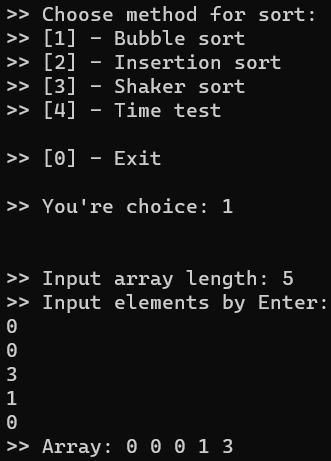
\includegraphics[scale=0.6]{screen_bubble_sort}}
    \caption{Тестирование сортировки пузырьком}
    \label{fig:image}
\end{figure}

\begin{figure}[h]
    \center{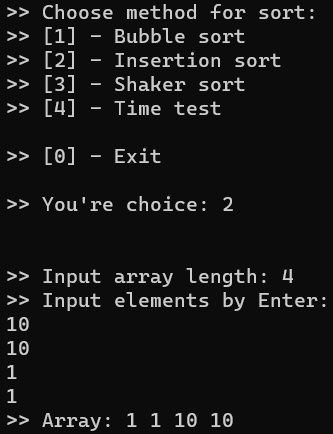
\includegraphics[scale=0.6]{screen_insertion}}
    \caption{Тестирование сортировки вставками}
    \label{fig:image}
\end{figure}

\begin{figure}[h]
    \center{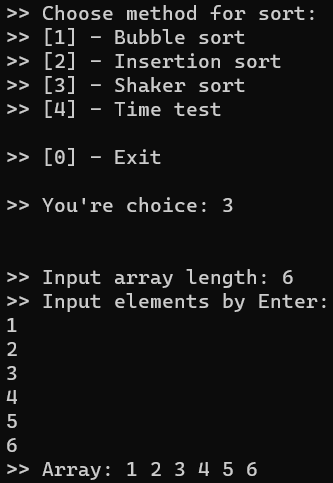
\includegraphics[scale=0.6]{screen_shaker}}
    \caption{Тестирование шейкерной сортировки}
    \label{fig:image}
\end{figure}

~
Все тесты прошли успешно.

\newpage
\section{Вывод}

По итогу, были реализованы функции алгоритмов сортировки массивов на языке C++, а также функции тестирования и подсчёта 
процессорного времени.

\newpage
\chapter{Исследовательская часть}

Измерения процессорного времени проводятся при одинаковых размерах массивов 100, 200, 300, 1000, 10000.

\section{Результаты экспериментов}

Проведя измерения процессорного времени выполнения реализованных алгоритмов, можно составить таблицу \ref{tabular:timesandtenses}.

\begin{table}[h]
\caption{Результаты замеров процессорного времени выполнения алгоритмов сортировки в секундах}
\label{tabular:timesandtenses}
\begin{center}
\begin{tabular}{ | l | l | l | l | l | l | }
\hline
    Название $\backslash$ Размер & 100                 & 200                 & 300                 & 1000                & 10000 \\ \hline
    Сорт. пузырьком              & $3.1 \cdot 10^{-5}$ & $1.1 \cdot 10^{-4}$ & $3.1 \cdot 10^{-4}$ & $2.6 \cdot 10^{-3}$ & 0.341 \\ \hline
    Сорт. вставками              & $8.1 \cdot 10^{-6}$ & $5.9 \cdot 10^{-5}$ & $5.2 \cdot 10^{-5}$ & $7.0 \cdot 10^{-4}$ & 0.071 \\ \hline
    Шейкерная сорт.              & $4.3 \cdot 10^{-5}$ & $1.4 \cdot 10^{-4}$ & $2.5 \cdot 10^{-4}$ & $2.5 \cdot 10^{-3}$ & 0.309 \\ \hline
\end{tabular}
\end{center}
\end{table}

\section{Вывод}

Анализируя результаты замеров затрачиваемого времени можно сказать, что самым быстрым алгоритмом, при использовании 
случайного заполнения, оказался алгоритм сортировки вставками, а алгоритм сортировки пузырьком и шейкерная сортировка 
являются разновидностями пузырьковой сортировки, следовательно результаты похожи. 
Однако на массивах большей длины выигрывает шейкерная сортировка.

\newpage
\chapter*{Заключение}
\addcontentsline{toc}{chapter}{Заключение}

В ходе работы были изучены алгоритмы сортировки массивов. 
Реализованы 3 алгоритма, приведен программный код реализации алгоритмов сортировки.
Была подсчитана трудоемкость каждого из алгоритмов, а также проведено сравнение алгоритмов по времени
 и трудоемкости. Показано, что наименее трудоемким и наименее затратным по времени алгоритмом является 
алгоритм сортировки вставками.\\

Цель работы достигнута, решены поставленные задачи.
Получены практические навыки реализации алгоритмов сортировки массивов, а также проведена 
исследовательская работа по вычислению трудоемкости алгоритмов и анализу их временных характеристик.

\newpage
\renewcommand\bibname{Список литературы}
\addcontentsline{toc}{chapter}{Список литературы}
\makeatletter % список литературы
\def\@biblabel#1{#1. }
\makeatother
\begin{thebibliography}{2}
    \bibitem{analyse1_info} Дж. Макконнелл. Анализ алгоритмов. Активный обучающий подход. -- М.: Техносфера, 2017. -- 267с.
    \bibitem{analyse2_info} Кормен Т. Алгоритмы: построение и анализ / Кормен Т. - Вильямс, 2014. - 198 с. - 219 с.
\end{thebibliography}

\end{document}

